\noindent\begin{minipage}{7cm}
\begin{description}
\item[Objectif :] comprendre la structure générale des boucles
pour mieux appréhender leur conception.
\item[Syntaxe \python :] \mbox{}\\
\texttt{while condition : blocWhile}
\end{description}
\end{minipage}
\mbox{}\hfill
\begin{tabular}{c}
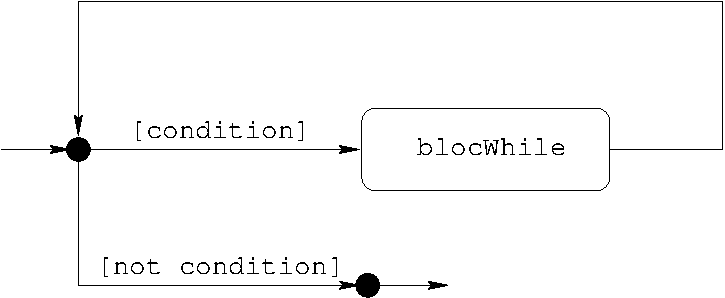
\includegraphics[width=6.5cm]{uml4.pdf}
\end{tabular}

%-------------------------------------------------------------------------
\subsection{Exemple}
%-------------------------------------------------------------------------

\paragraph{Enoncé}
On dispose d'une planche, d'un marteau et d'un clou (situation initiale)
et on veut que le clou soit enfoncé dans la planche jusqu'à  la tête (situation finale).

\paragraph{Méthode}
Le travail à  réaliser consiste donc à  planter légèrement le clou
à  la main de faà§on qu'il tienne seul, puis à  taper sur la tête du 
clou avec le marteau tant que la tête ne touche pas la planche. 
Le nombre de coups nécessaire est \emph{a priori} inconnu.


\paragraph{Questions} 
Le passage de la compréhension intuitive d'un
tel énoncé à  l'algorithme n'est pas toujours facile à  réaliser. 
Pour nous y aider, nous introduisons 4 notions : 
l'initialisation, l'invariant, la progression et la condition d'arrêt.

\begin{question}[« planter un clou » : initialisation] 
Par quelle opération commence-t-on pour «~enfoncer le clou » ? 
Il s'agit de l'initialisation du processus « planter un clou ».
\end{question}


\begin{question}[« planter un clou » : progression] 
Une fois l'initialisation réalisée,
quelle opération doit-on effectuer pour atteindre la situation finale ?
Cette opération doit faire progresser le système vers sa situation finale.
\end{question}


\begin{question}[« planter un clou » : invariant] 
Au cours de la progression du processus d'enfonce\-ment du clou,
une situation est toujours vérifiée. Laquelle ? 
On parle d'invariant du processus.
\end{question}


\begin{question}[« planter un clou » : condition d'arrêt] 
A quelle condition a-t-on atteint la situation finale ? 
Il s'agit de la condition d'arrêt du processus.
\end{question}

L'invariant et la condition d'arrêt définissent des situations
tandis que l'initialisation et la progression concernent des actions. 
On notera les situations entre crochets (\texttt{[situation]}) pour les distinguer 
des actions (\texttt{« action »}).

\begin{question}[« planter un clou » : algorithme] 
Disposant maintenant des 4 notions précédentes
(l'initialisation, l'invariant, la progression et la condition d'arrêt), 
proposer un algorithme pour «~planter un clou ».
\end{question}


%-------------------------------------------------------------------------
\subsection{Généralisation}
%-------------------------------------------------------------------------
Un algorithme est un mécanisme qui fait passer un « système » d'une « situation »
dite initiale (ou \texttt{[précondition]}) à  une « situation » finale 
(\texttt{[postcondition]} ou \texttt{[but]}). 
Le couple (situation initiale, situation finale) constitue une spécification de 
l'algorithme. 
L'algorithmique vise alors à  construire rationnellement des algorithmes à  partir de 
leur spécification.

Dans le cas d'une boucle, la construction de l'algorithme passe par les 
4 étapes suivantes :
\begin{enumerate}
\item {\bf Invariant :} proposer une situation générale décrivant le problème posé. 
	Cette étape est la plus délicate car elle exige de faire 
	preuve d'imagination.

	Notation : \texttt{[invariant]}
	
\item {\bf Condition d'arrêt :} à  partir de la situation générale imaginée en [1], 
	on doit formuler la condition qui permet d'affirmer que l'algorithme a 
	terminé son travail. 
	La situation dans laquelle il se trouve alors est appelée situation finale.
	La condition d'arrêt fait sortir de la boucle.

	Notation : \texttt{[condition d'arrêt]}
	
\item {\bf Progression :} se « rapprocher » de la situation finale, tout en faisant 
	le nécessaire pour conserver à  chaque étape une situation générale 
	analogue à  celle retenue en [1].
	La progression conserve l'invariant.

	Notation : \texttt{« progression »}
	
\item {\bf Initialisation :} initialiser les variables introduites dans l'invariant 
	pour que celui-ci soit vérifié avant d'entrer dans la boucle.
	L'initialisation « instaure » l'invariant.

	Notation : \texttt{« initialisation »}
	
\end{enumerate}

\begin{question}[construction d'une boucle : initialisation et invariant] 
Dans l'exemple « planter un clou », vérifier que l'initialisation instaure 
l'invariant.
\end{question}

\begin{question}[construction d'une boucle : condition d'arrêt et invariant] 
Dans l'exemple du \linebreak clou, montrer à  l'aide d'un contre-exemple
qu'il ne suffit pas de vérifier la condition d'arrêt pour que la situation 
finale recherchée soit atteinte.
\end{question}

\begin{question}[construction d'une boucle : cas général] 
Proposer la structure générale d'une bou\-cle en combinant les 4 étapes précédentes.
Dessiner le diagramme \textsc{Uml} correspondant.\\
Vérifier que l'algorithme « planter un clou » a bien cette structure générale.
\end{question}

\begin{question}[construction d'une boucle : cas simplifié] 
Dans la pratique, on utilise une simplification du cas général précédent.
Laquelle ?
Dessiner le diagramme \textsc{Uml} correspondant.\\
Simplifier en conséquence l'algorithme « planter un clou ».
\end{question}

Cette façon de procéder permet de « prouver » la validité de l'algorithme au fur et à 
mesure de son élaboration. 
En effet la situation générale choisie en [1] est en fait l'invariant 
qui caractérise la boucle {\tt while}.
Cette situation est satisfaite au départ grace à  l'initialisation de l'étape [4]; 
elle reste vraie à  chaque itération (étape [3]). Ainsi lorsque la condition d'arrêt 
(étape [2]) est atteinte, cette situation nous permet d'affirmer que le problème 
est résolu. C'est également en analysant l'étape [3] qu'on peut prouver la 
terminaison de l'algorithme.

%-------------------------------------------------------------------------
\subsection{Applications}
%-------------------------------------------------------------------------
\begin{question}[construction d'une boucle : fonction puissance] 
Ecrire l'algorithme de calcul de la fonction puissance ($x^p$) en
définissant l'initialisation, l'invariant, la progression et la condition d'arrêt
correspondants.
\end{question}

\begin{question}[construction d'une boucle : fonction factorielle] 
Ecrire l'algorithme de calcul de la fonction factorielle ($n!$) en
définissant l'initialisation, l'invariant, la progression et la condition d'arrêt
correspondants.
\end{question}

\begin{question}[construction d'une boucle : fonction pgcd] 
Ecrire un algorithme qui calcule le plus grand commun diviseur (pgcd) de deux
nombres en définissant l'initialisation, l'invariant, la progression et la condition d'arrêt
correspondants.
\end{question}

\begin{question}[construction d'une boucle : fonction Fibonacci] 
L'algorithme suivant permet de calculer le nombre $f$ de Fibonacci à  l'ordre $n$.\\
\noindent\begin{minipage}{9cm}
Retrouver l'initialisation, l'invariant, la progression et la condition d'arrêt
qui ont permis de construire cet algorithme.
\end{minipage}
\hfill
\begin{minipage}{4.5cm}\footnotesize\tt
\begin{Verbatim}[frame=single]
i, f, f1, f2 = 3, 2, 1, 1
while i < n + 1 :
    f2 = f1
    f1 = f
    f = f1 + f2
    i = i + 1
\end{Verbatim}
\end{minipage}
\end{question}

%%-------------------------------------------------------------------------
%\subsection{QCM}
%%-------------------------------------------------------------------------
%\begin{enumerate}
%\item L'itération conditionnelle est une instruction
%	\begin{enumerate}
%	\item qui permet d'exécuter une instruction sous condition préalable.
%	\item qui est vérifiée tout au long de son exécution. 
%	\item qui permet sous condition préalable de répéter zéro ou plusieurs fois la même instruction.
%	\item qui permet de choisir entre plusieurs instructions.
%	\end{enumerate}
%\item On ne sort jamais d'une boucle si la condition d'arrêt 
%	\begin{enumerate}
%	\item ne varie pas en cours d'exécution.
%	\item ne contient pas d'opérateurs booléens.
%	\item est toujours fausse.
%	\item n'est jamais fausse.
%	\end{enumerate}
%\item Un invariant de boucle est une propriété 
%	\begin{enumerate}
%	\item vérifiée uniquement en début de boucle
%	\item vérifiée uniquement en fin de boucle
%	\item toujours fausse tout au long de l'exécution de la boucle.
%	\item vérifiée tout au long de l'exécution de la boucle.
%	\end{enumerate}
%\item Que vaut {\tt f} à  la fin des instructions suivantes si $n = 6$ ?
%	\hfill\begin{minipage}[t]{4.5cm}\footnotesize
%\begin{Verbatim}[frame=single]
%i, f, f1, f2 = 3, 2, 1, 1
%while i < n + 1 :
%    f2 = f1
%    f1 = f
%    f = f1 + f2
%    i = i + 1
%\end{Verbatim}
%	\end{minipage}
%
%	\begin{enumerate}
%	\item 5
%	\item 8
%	\item 13
%	\item 21
%	\end{enumerate}
%
%\end{enumerate}

%-------------------------------------------------------------------------
%\newpage
\subsection{Entraînement}
%-------------------------------------------------------------------------

%-------------------------------------------------------------------------
\subsubsection{Enoncé}
%-------------------------------------------------------------------------

\paragraph{Objectif :} 
écrire un algorithme qui calcule $y = f(x)$ en fonction du développement en série entière de la fonction $f$ : 
$f(x) = \sum u_k$, en respectant les contraintes suivantes :
\begin{itemize}
\item les calculs seront arrêtés lorsque la valeur absolue du terme $u_k$ ($|u_k|$) 
	sera inférieure à un certain seuil $s$ (avec $0 < s < 1$);
\item on n'utilisera ni la fonction \emph{puissance} ($x^n$) ni la fonction
	\emph{facto\-riel\-le} ($n!$) pour effectuer le calcul du développement.
\end{itemize}

\paragraph{Méthode :} construire l'algorithme en définissant l'initialisation, 
l'invariant, la progression et la condition d'arrêt correspondants.

\paragraph{Vérification :} vérifier avec \python{} les résultats obtenus pour 
différentes valeurs de $x$ en les comparant aux calculs directs de la fonction $f(x)$.

%\paragraph{Mots-clés:} itération, boucle \texttt{while}.

%-------------------------------------------------------------------------
\subsubsection{Exemple}
%-------------------------------------------------------------------------
\noindent 
On veut calculer $\forall x \in ]-1;1[$ la fonction $f(x)$ définie par 
$$\begin{array}{lll}
\displaystyle y = f(x) = \frac{1}{(1+x)^a} & \approx &\displaystyle  1 + \sum_{k=1}^{n} u_k  = 1 + \sum_{k=1}^{n} (-1)^k a(a+1)\cdots(a+k-1)\frac{x^k}{k!}\\
	           & = &\displaystyle 1 - ax + a(a+1)\frac{x^2}{2} + \ldots +
(-1)^k a(a+1)\cdots(a+k-1)\frac{x^k}{k!}
\end{array}$$
On cherche une relation de récurrence $g$ entre $u_{k+1}$ et $u_k$ afin de faciliter le calcul de $u_{k+1}$ 
sans faire appel aux fonctions \emph{puissance} ($x^{k}$) et \emph{factorielle} ($k!$).

$$\begin{array}{lll}
\multicolumn{3}{l}{\mbox{On a :}} \\
\displaystyle u_{k+1} &=& \displaystyle (-1)^{k+1} a(a+1)\cdots(a+(k+1)-1)\frac{x^{k+1}}{(k+1)!} \\
\multicolumn{3}{l}{\mbox{et on cherche donc à faire apparaître $u_k$ dans l'expression de $u_{k+1}$ :}}\\
\displaystyle u_{k+1} &=& \displaystyle (-1)\cdot(-1)^k\cdot a(a+1)\cdots(a+k-1)\cdot(a+k)\cdot\frac{x\cdot x^k}{k!(k+1)}\\
\displaystyle u_{k+1} &=& \displaystyle - x\cdot\frac{(a+k)}{(k+1)}\cdot (-1)^k a(a+1)\cdots(a+k-1)\frac{x^k}{k!} = \displaystyle - x\cdot\frac{(a+k)}{(k+1)}\cdot u_k
= g(u_k)
\end{array}$$

Ainsi, dans la pratique, si on mémorise la valeur de $u_k$, on calculera sans problème 
la valeur de $u_{k+1}$ grâce à cette relation de récurrence ($u_{k+1} = g(u_k)$).
$$\begin{array}{lllllll}
y_1     &=& 1 + u_1 \\
y_2     &=& 1 + u_1 + u_2                          &=& y_1 + u_2         &=& y_1 + g(u_1) \\
y_3     &=& 1 + u_1 + u_2 + u_3                    &=& y_2 + u_3         &=& y_2 + g(u_2)\\
\multicolumn{7}{l}{\ldots}\\
y_{m+1} &=& 1 + u_1 + u_2 + \cdots + u_m + u_{m+1} &=& y_{m} + u_{m+1}   &=& y_m + g(u_{m})
\end{array}$$

\paragraph{Méthode} 
Les 4 étapes de construction de l'algorithme recherché sont donc les suivantes :
\begin{itemize}
\item pour l'invariant, on vérifie qu'à chaque étape $m$, $y$ est toujours égal à la somme 
	des $m$ premiers termes $u_k$ : 
	$\displaystyle \forall m, y_m = 1 + \sum_{k=1}^m u_k$;
\item l'initialisation consiste à décrire le cas $m = 1$ : 
	$u_1 = -ax$ et $y = y_1 = 1 + u_1 = 1 - ax$;
\item la progression consiste à calculer l'étape suivante à partir de l'étape courante ($m \rightarrow m+1$) :\\
	$\displaystyle u_{m+1} = g(u_m) = - x\cdot\frac{(a+m)}{(m+1)}\cdot u_{m}$, $y_{m+1} = y_{m} + g(u_{m})$;
\item la condition d'arrêt est contrainte par l'énoncé : 
	$|u_m| < s$.
\end{itemize}
\vspace*{3mm}

\noindent L'algorithme recherché prendra la forme :\\
\begin{minipage}[t]{8cm}
\begin{Verbatim}
« initialisation »
while not « condition d'arrêt » :
    « progression »
\end{Verbatim}
\end{minipage}
\hfill
\begin{minipage}[t]{7cm}\footnotesize
$m = 1$, $u_1 = -ax$, $y_1 = 1 - ax$\\
\texttt{while not} $|u_m| < s$ \texttt{:}\\
\mbox{}\texttt{\ \ \ \ } $u_{m+1} = g(u_m)$\\
\mbox{}\texttt{\ \ \ \ } $y_{m+1} = y_{m} + u_{m+1}$\\
\mbox{}\texttt{\ \ \ \ } $m \rightarrow m+1$
\end{minipage}

\noindent
\begin{minipage}[t]{7cm}
\paragraph{Résultat} En \python, l'algorithme correspondant est présenté
ci-contre.
Pour le tester, on fixera différentes valeurs des données $a$, $x$ et $s$,
et pour le vérifier, on comparera la valeur $y$ calculée 
avec le calcul direct $(1+x)^{-a}$.
\end{minipage}
\hfill
\begin{minipage}[t]{8cm}
\begin{lstlisting}
m = 1
u = -a*x
y = 1 + u
while not fabs(u) < s :
    u = -u*x*(a + m)/(m + 1)
    y = y + u
    m = m + 1
\end{lstlisting}
\end{minipage}

\paragraph{Vérifications} on compare le résultat obtenu par l'algorithme avec 
le calcul direct : $\displaystyle y - \frac{1}{(1+x)^a}$, 
pour différentes valeurs des données $a$, $x$ et $s$.
\vspace*{3mm}

\noindent
\begin{minipage}[t]{7cm}\footnotesize
\begin{Verbatim}
>>> a, x, s = 1, 0, 1.0e-9
...
>>> y - 1/(1-x)**a
0.0

>>> a, x, s = 1/2, 0.5, 1.0e-9
...
>>> y - 1/(1-x)**a
-2.65160005064e-10

>>> a, x, s = 3, 0.5, 1.0e-9
...
>>> y - 1/(1-x)**a
2.69446243095e-10
\end{Verbatim}
\end{minipage}
\hfill
\begin{minipage}[t]{7cm}\footnotesize
\begin{Verbatim}
>>> a, x, s = 5, 0, 1.0e-9
...
>>> y - 1/(1-x)**a
0.0

>>> a, x, s = 5, 0.85, 1.0e-9
...
>>> y - 1/(1-x)**a
4.27782663459e-10

>>> a, x, s = 5, -0.85, 1.0e-9
...
>>> y - 1/(1-x)**a
-5.8480509324e-09
\end{Verbatim}
\end{minipage}
%\vspace*{5mm}

\newpage
\noindent
\begin{minipage}[t]{7cm}\footnotesize
\begin{Verbatim}
>>> a, x, s = 3, 0.5, 1.0e-4
...
>>> y - 1/(1-x)**a
2.31884143971e-05
\end{Verbatim}
\end{minipage}
\hfill
\begin{minipage}[t]{7cm}\footnotesize
\begin{Verbatim}
>>> a, x, s = 5, -0.85, 1.0e-5
...
>>> y - 1/(1-x)**a
-6.00809507887e-05
\end{Verbatim}
\end{minipage}
\vspace*{5mm}

\noindent
Les différences observées sont toutes voisines de 0 et compatibles
avec le seuil de précision $s$ donné.


%-------------------------------------------------------------------------
%\newpage
\subsubsection{Questions}
%-------------------------------------------------------------------------
\begin{enumerate}
\item $\displaystyle \exp(x) \approx \sum_{k=0}^{n} \frac{x^{k}}{k!} = 1 + x + \frac{x^2}{2} + \cdots + \frac{x^{n}}{n!}$\hfill$\forall x \in \mathbb{R}$
\item $\displaystyle \exp(-x) \approx \sum_{k=0}^{n} (-1)^k\frac{x^{k}}{k!} = 1 - x + \frac{x^2}{2} + \cdots + (-1)^n\frac{x^{n}}{n!}$\hfill$\forall x \in \mathbb{R}$
\item $\displaystyle\log(1+x) \approx \sum_{k=1}^{n} (-1)^{k+1}\frac{x^k}{k} = x - \frac{x^2}{2} + \frac{x^3}{3} + \cdots + (-1)^{n+1}\frac{x^n}{n}$ \hfill$\forall x \in ]-1;1]$
\item $\displaystyle\log(1-x) \approx \sum_{k=1}^{n} -\frac{x^k}{k} = -x -\frac{x^2}{2} - \frac{x^3}{3} -\cdots - \frac{x^n}{n}$ \hfill$\forall x \in [-1;1[$
\item $\displaystyle\log\left(\frac{1+x}{1-x}\right) = 2 \sum_{k=0}^{n} \frac{x^{2k+1}}{2k+1} = $\hfill$\forall x \in [-1;1[$
\item $\displaystyle\sinh(x) \approx \sum_{k=0}^{n} \frac{x^{2k+1}}{(2k+1)!} = x + \frac{x^3}{6} + \frac{x^5}{120} + \cdots + \frac{x^{2n+1}}{(2n+1)!}$\hfill$\forall x \in \mathbb{R}$
\item $\displaystyle\cosh(x) \approx \sum_{k=0}^{n} \frac{x^{2k}}{(2k)!} = 1 + \frac{x^2}{2} + \frac{x^4}{24} + \cdots + \frac{x^{2n}}{(2n)!}$\hfill$\forall x \in \mathbb{R}$
\item $\displaystyle\arg\sinh(x) \approx x + \sum_{k=1}^{n}  (-1)^k \frac{1\times 3\times\cdots\times (2k-1)}{2\times 4\cdots\times 2k}\frac{x^{2k+1}}{2k+1} =\\  x - \frac{1}{2} \frac{x^3}{3} + \frac{1}{2} \frac{3}{4} \frac{x^5}{5} - \frac{1}{2} \frac{3}{4} \frac{5}{6}\frac{x^7}{7} + \cdots + (-1)^n \frac{1\times 3\times\cdots\times (2n-1)}{2\times 4\cdots\times 2n}\frac{x^{2n+1}}{2n+1}$ \hfill$\forall x \in ]-1;1[$  
\item $\displaystyle\arg\tanh(x) \approx \sum_{k=0}^{n} \frac{1}{2k+1}x^{2k+1} = x + \frac{x^3}{3} + \frac{x^5}{5}\cdots + \frac{1}{2n+1}x^{2n+1}$\hfill$\forall x \in ]-1;1[$  	
\item $\displaystyle\sin(x) \approx \sum_{k=0}^{n} (-1)^k\frac{x^{2k+1}}{(2k+1)!} = 		x - \frac{x^3}{6} + \frac{x^5}{120} + \cdots + (-1)^n\frac{x^{2n+1}}{(2n+1)!}$\hfill$\forall x \in \mathbb{R}$
\item $\displaystyle\cos(x) \approx \sum_{k=0}^{n} (-1)^k\frac{x^{2k}}{(2k)!} =         1 - \frac{x^2}{2} + \frac{x^4}{24} + \cdots + (-1)^n\frac{x^{2n}}{(2n)!}$\hfill$\forall x \in \mathbb{R}$
\item $\displaystyle\arcsin(x) \approx x + \sum_{k=1}^{n} \frac{1\times 3\times\cdots\times (2k-1)}{2\times 4\cdots\times 2k}\frac{x^{2k+1}}{2k+1} =\\ x + \frac{1}{2} \frac{x^3}{3} + \frac{1}{2}\frac{3}{4}\frac{x^5}{5} + \frac{1}{2} \frac{3}{4} \frac{5}{6}\frac{x^7}{7} + \cdots + \frac{1\times 3\times\cdots\times (2n-1)}{2\times 4\cdots\times 2n}\frac{x^{2n+1}}{2n+1}$ \hfill$\forall x \in ]-1;1[$ 
\item $\displaystyle\arccos(x) \approx \frac{\pi}{2} - x - \sum_{k=1}^{n} \frac{1 \cdot 3 \cdot 5 \cdots (2k-1) x^{2k+1}}{2 \cdot 4 \cdot 6 \cdots (2k) \cdot (2k+1)} = \\ \frac{\pi}{2} - x - \frac{x^3}{2 \cdot 3} - \frac{1 \cdot 3 \cdot x^5}{2 \cdot 4 \cdot 5} - \cdots - \frac{1 \cdot 3 \cdot 5 \cdots (2n-1) x^{2n+1}}{2 \cdot 4 \cdot 6 \cdots (2n) \cdot (2n+1)} $\hfill$\forall x \in ]-1;1[$
\item $\displaystyle\arctan(x) \approx \sum_{k=0}^{n} (-1)^k \frac{x^{2k+1}}{(2k+1)} = x - \frac{x^3}{3} + \frac{x^5}{5} + \cdots + (-1)^n \frac{x^{2n+1}}{(2n+1)}$\hfill$\forall x \in \mathbb{R}$
\item $\displaystyle \frac{1}{1+x} \approx \sum_{k=0}^{n} (-1)^k x^k = 1 - x + x^2 - x^3 + \cdots + (-1)^n x^n$\hfill$\forall x \in ]-1;1[$  
\item $\displaystyle \frac{1}{1-x} \approx \sum_{k=0}^{n} x^k = 1 + x + x^2 + x^3 + \cdots + x^n$\hfill$\forall x \in ]-1;1[$
\item $\displaystyle \frac{1}{1+x^2} \approx \sum_{k=0}^{n} (-1)^k x^{2k} = 1 - x^2 + x^4 + \cdots + (-1)^n x^{2n}$\hfill$\forall x \in ]-1;1[$  
\item $\displaystyle \frac{1}{1-x^2} \approx \sum_{k=0}^{n} x^{2k} = 1 + x^2 + x^4 + \cdots + x^{2n}$\hfill$\forall x \in ]-1;1[$
\item $\displaystyle \sqrt{1+x} \approx 1 + \frac{x}{2} + \sum_{k=2}^{n} (-1)^{k-1} \frac{1\times3\times\cdots\times(2k-3)}{2^k} \frac{x^k}{k!} =\\ 1 + \frac{x}{2} - \frac{x^2}{8} + \frac{x^3}{16} - \frac{5x^4}{128} + \cdots + (-1)^{n-1} \frac{1\times3\times\cdots\times(2n-3)}{2^n} \frac{x^n}{n!} $\hfill$\forall x \in ]-1;1[$
\item $\displaystyle \frac{1}{\sqrt{1+x}} \approx 1 + \sum_{k=1}^{n} (-1)^k \frac{1\times 3\times\cdots\times (2k-1)}{2\times 4\cdots\times 2k} x^k =\\ 1 - \frac{1}{2} x + \frac{1}{2}\frac{3}{4} x^2 - \frac{1}{2}\frac{3}{4}\frac{5}{6} x^3 + \cdots + (-1)^n \frac{1\times 3\times\cdots\times (2n-1)}{2\times 4\cdots\times 2n} x^n$ \hfill$\forall x \in ]-1;1[$
\item $\displaystyle \frac{1}{\sqrt{1-x^2}} \approx \sum_{k=0}^{n} \frac{(2k)!}{2^{2k}(k!)^2} x^{2k} = 1 + \frac{x^2}{2} + \frac{3x^4}{8} + \cdots +  \frac{(2n)!}{2^{2n}(n!)^2} x^{2n}$ \hfill$\forall x \in ]-1;1[$
\item $\displaystyle \frac{1}{(a-x)^2} \approx \sum_{k=0}^{n} \frac{k+1}{a^{k+2}}x^k = \frac{1}{a^2} \left( 1 + \frac{2x}{a} + \frac{3x^2}{a^2} + \cdots + \frac{(n+1)x^n}{a^n}\right)$\hfill$\forall x \in ]-|a|;|a|[$
\item $\displaystyle \frac{1}{(a-x)^3} \approx \sum_{k=0}^{n} \frac{(k+1)(k+2)}{2a^{k+3}}x^k =\\ \frac{1}{a^3} \left( 1 + \frac{3x}{a} + \frac{6x^2}{a^2} + \cdots + \frac{(n+1)(n+2)}{2a^{n}}x^n \right)$\hfill$\forall x \in ]-|a|;|a|[$
\item $\displaystyle \frac{1}{(a-x)^5} \approx \sum_{k=0}^{n} \frac{(k+1)(k+2)(k+3)(k+4)}{24a^{k+5}}x^k =\\ \frac{1}{a^5} \left( 1 + \frac{5x}{a} + \frac{15x^2}{a^2} + \cdots + \frac{(n+1)(n+2)(n+3)(n+4)}{24a^{n}}x^n \right)$\hfill$\forall x \in ]-|a|;|a|[$
\end{enumerate}

%-------------------------------------------------------------------------
\subsection{Révisions}
%-------------------------------------------------------------------------

$$\begin{tabular}{|ll@{ : }l|}
\hline
\textbf{Cours} & \cite{cours} & chapitre 2, sections 2.4.1 et 2.6.3 \\
\textbf{TD}    & \cite{td}    & exercices 2.12 à  2.16, 2.33, 2.40, 2.44 et 2.45 \\
\hline
\end{tabular}$$
